\documentclass{article}
\usepackage{graphicx}
\usepackage{geometry}
\usepackage{fancyhdr}										% Headers and footers
\usepackage{xcolor}											% Better colors
\usepackage{xpatch}											% Better macro patches
\usepackage{hyperref}										% Hyperlinks
\usepackage{fontspec}										% Custom fonts
\usepackage{tikz}											% Graphics creation
\usepackage{float}											% Figure positioning
\usepackage{tabu}											% Better tables
\usepackage[font={small,it}]{caption}						% Italic captions
\usepackage{listings}
\geometry{left=1in,right=1in,top=1in,bottom=1in}

\hypersetup{
	colorlinks=true,
	linkcolor=black
}

%************************************************%
\title{Lab 2 Report}
\author{Jinzhi Cai, Ryan Kane, Yifei Che}
\date{\today}
%************************************************%


\makeatletter
\begin{document}
	\maketitle
	\newpage
	\tableofcontents
	\clearpage
	\section{Introduction}
	Embedded system play an important role in the modern society. In this lab, we will discuss how to create an embedded system using open source hardware and learn about the different problem engineers will facing in the real life development.
	\section{Boot and display the Beaglebone Desktop GUI}
	\subsection{Setup}
	In this experiment of the lab, we will upload a system image with a graphical user interface onto the Beaglebone Black. The setup for this experiment includes having a microSD card with at least 4GB of storage, a usb keyboard and mouse, and an HDMI cable.
	
	\subsection{Procedure}
	First, the latest GUI system image can be obtained at https://beagleboard.org/latest-images. Here the system image downloaded is the “Debian X.X 4GB SD LXQT”. After the image is downloaded, it has to be extracted from an .img.xz file to a .img file. After this is done, the image is then flashed to the SD card using Etcher. In Etcher select the SD Card, press flash and wait for the process to finish. Now, make sure the board is powered down by unplugging it from the computer if it is plugged in. Then insert the SD card and plug it back into the computer while holding the user button until it is booted successfully. 
	
	
	\subsection{Result}
	After the board is booted properly, it should display on the monitor through the HDMI cable, and can be controlled using a plugged in keyboard and mouse \ref{BBD}. 
	
	\begin{figure}[hb]
		\centering
		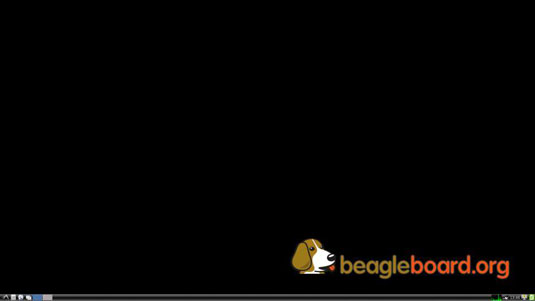
\includegraphics[width=0.5\textwidth]{img/Lab2_beaglebone_DP.jpg}
		\caption{Beaglebone Desktop} 
		\label{BBD}
	\end{figure}
	\clearpage
	\section{Boot and display the RPi Desktop}
	\subsection{Setup}
	Now, we will setup the Raspberry Pi Zero with a system image that will be used for the remainder of the lab. For this setup, a Raspberry Pi Zero and a microSD card with at least 4GB is needed.
	
	\subsection{Procedure}
	First, the latest system image can be obtained at https://www.raspberrypi.org/downloads/raspbian/. Here, any system image can be downloaded, but the lighter the image the faster it will run. We selected the lightest version that only has terminal support. After the image is downloaded, it has to be extracted from an .zip file to a .iso file. After this is done, the image is then flashed to the SD card using Etcher. In Etcher select the SD Card, press flash and wait for the process to finish. Now, make sure the board is powered down by unplugging it from the pi if it is plugged in. Then insert the SD card and plug it back into the pi.
	
	\subsection{Result}
	After the board is booted properly, it should display on the monitor through the HDMI cable (terminal or GUI depending on the system image), and can be controlled using a plugged in keyboard and mouse \ref{RBD}. 
	\begin{figure}[hb]
		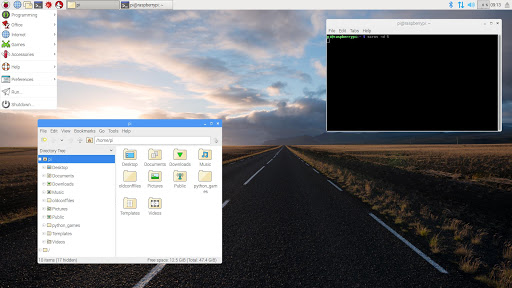
\includegraphics[width=\textwidth]{img/Lab2_RBP_DP.jpg}
		\caption{Raspberry Desktop} 
		\label{RBD}
	\end{figure}
	\clearpage
	\section{Arduino serial port}
	\subsection{Setup}
	For this task, we will encode a packet using COBS format to make our communication protocol more robust. The setup required is connecting the TX pin on the Adafruit ItzyBitzy M0 to the Analog Discovery pin 0. Then, make sure the PacketSerial library is installed for the Arduino IDE.
	
	\subsection{Procedure}
	First, The PacketSerial library is imported and a handler for it is created. Then we create a packet, which is a uint8\_t array to send out the serial port. This is done by calling the send() method of the PacketSerial object. This method takes the array and encodes it using the COBS format and sends it out the serial port. The full code for this experiment can be found in the appendix.
	
	\subsection{Result}
	Using the Analog Discovery, a UART receiver can be setup in the Logic window. Here we can see the packet sent is now encoded into COBS format, with an extra padding byte in front, and a 0 byte at the end.
	
	\clearpage
	\section{Flip a bit test on RPi}
	\subsection{Setup}
	Since we are unable to type gpio in the command line in the first place, we have to connect to the WIFI and download the image which has the wiring Pi library. Then we install the wiring Pi. For hardware setup, we connect the ground (on analog discovery side) to raspberry pi, and 1+(analog discovery side) to gpio pin 7.
	\subsection{Procedure}
	In the C++ code, we define the LED 7 first. In the main function, we start with the wiringPiSetup() function, which can initialize the wiring Pi and we can further use the scheme. The next line “pinMode(LED, OUTPUT)” set the pin 7 to output pin mode. Then, we have a while loop that goes forever. In the while loop, we use the DigitalWrite(LED,1) and DigitalWrite(LED,0) repeatedly so that we can continuously change send 1 and 0 to make the bit flipped. 
	\subsection{Result}
	We use the analog discovery to detect the signal sent from Raspberry Pi. The frequency is set to 6.4MHz. We can see the bit flipping between 0 and 1.
	\begin{figure}[hb]
		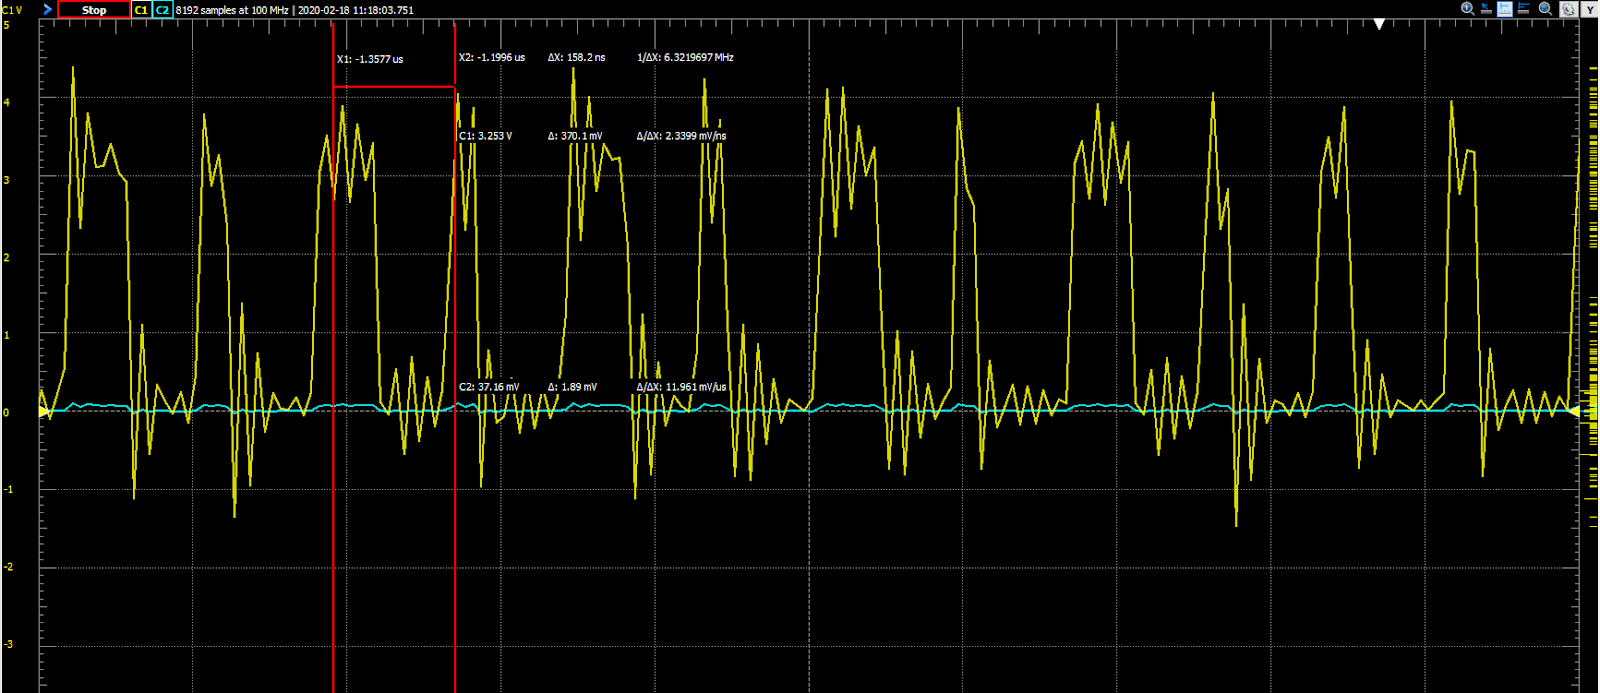
\includegraphics[width=\textwidth]{img/Lab3_FlipaBit.PNG}
		\caption{Analog Discovery Scope for Raspberry Pi Bit} 
		\label{CNN5}
	\end{figure}
	\clearpage
	\section{Send serial data to and from RPi from Arduino}
	\subsection{Setup}
	Since we are unable to type gpio in the command line in the first place, we have to connect to the WIFI and download the image which has the wiring Pi library. Then we install the wiring Pi. For hardware setup, we connect the ground (on analog discovery side) to raspberry pi, and 1+(analog discovery side) to gpio pin 7\ref{CNN5}.
	\begin{figure}[hb]
		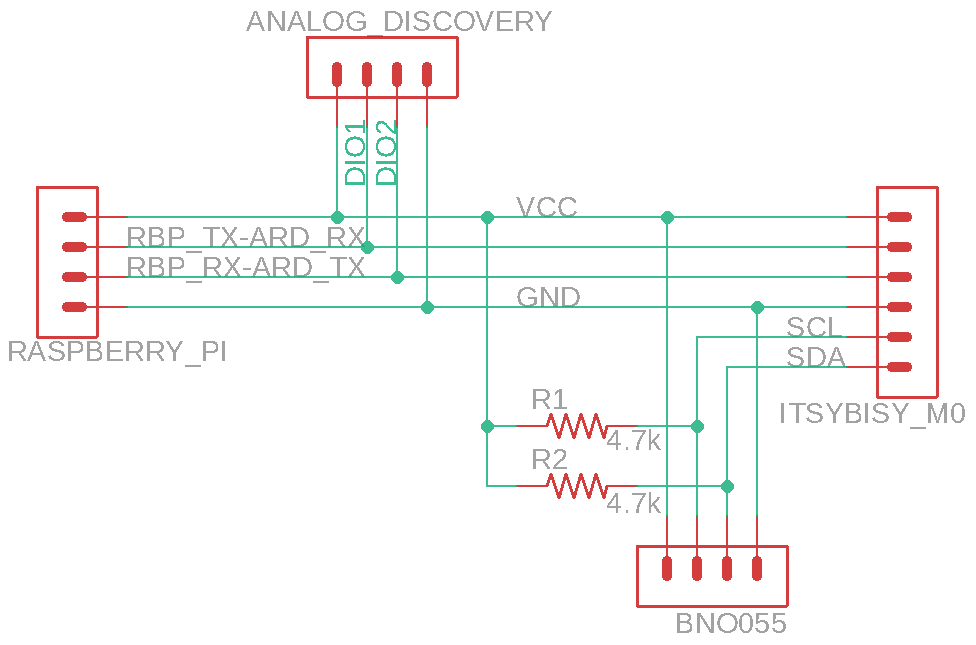
\includegraphics[width=\textwidth]{img/Lab3_SerialConnection.png}
		\caption{Circuit Diagram For Serial Connection} 
		\label{CNN5}
	\end{figure}
	
	\subsection{Procedure}
	In the C++ code, we define the LED 7 first. In the main function, we start with the wiringPiSetup() function, which can initialize the wiring Pi and we can further use the scheme. The next line “pinMode(LED, OUTPUT)” set the pin 7 to output pin mode. Then, we have a while loop that goes forever. In the while loop, we use the DigitalWrite(LED,1) and DigitalWrite(LED,0) repeatedly so that we can continuously change send 1 and 0 to make the bit flipped.
	
	\subsection{Result}
	We use the analog discovery to detect the signal sent from Raspberry Pi. The frequency is set to 6.4MHz. We can see the bit flipping between 0 and 1.
	
	\clearpage
	\section{Send a single float in COBS format out Arduino}
	\subsection{Setup}
	For this task, we will encode a packet using COBS format to make our communication protocol more robust. The setup required is connecting the TX pin on the Adafruit ItzyBitzy M0 to the Analog Discovery pin 0. Then, make sure the PacketSerial library is installed for the Arduino IDE.
	\subsection{Procedure}
	First, The PacketSerial library is imported and a handler for it is created. Then we create a packet, which is a uint8\_t array to send out the serial port. This is done by calling the send() method of the PacketSerial object. This method takes the array and encodes it using the COBS format and sends it out the serial port. The full code for this experiment can be found in the appendix.
	\subsection{Result}
	Using the Analog Discovery, a UART receiver can be setup in the Logic window. Here we can see the packet sent is now encoded into COBS format, with an extra padding byte in front, and a 0 byte at the end.
	\clearpage
	\section{Send a single float in COBS format, A to RPi}
	\subsection{Setup}
	For this task, we now will convert the Arduino code to read an Analog voltage from an potentiometer, and send it to the Raspberry Pi in COBS format. To set it up, we connect the middle pin of the potentiometer to pin A1 on the Arduino, and connect the other two to 5V and GND \ref{CNN3}.
	\begin{figure}[hb]
		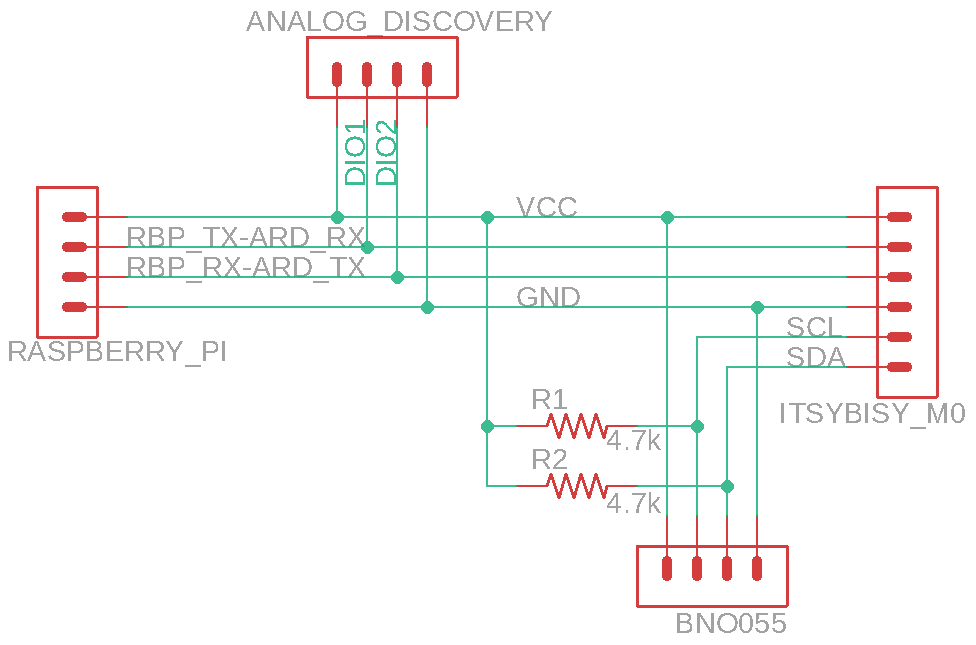
\includegraphics[width=\textwidth]{img/Lab3_SerialConnection.png}
		\caption{Circuit Diagram For Serial Connection} 
		\label{CNN3}
	\end{figure}
	
	\subsection{Procedure}
	For the Arduino code, we first loop to read the analog voltage on pin A1 and scale it based on a 1024 bit ADC and a max voltage of 3 volts. Now, since the PacketSerial method uses uint8\_t arrays to send the data, we must define a union to convert the float value to an array of integers (length of 4). Using this union, we assign the float of it to the reading from the ADC. Then, we send the integer array in the send() method. Now, on the Raspberry Pi this value is read by the SerialHandler class, and then decoded using the COBSHandler class.Finally, the union is reversed on the Raspberry Pi side and we are left with the float that was sent by the Arduino. The Arduino code can be found in Appendix B.
	
	\subsection{Result}
	Using the potentiometer to send different voltages to the Arduino correctly changes the value outputted by the Raspberry Pi, with a small delay as the communication and processing occurs.
	
	\clearpage
	\section{Send a float array in COBS format, A to RPi}
	\subsection{Setup}
	In this task, we adapt the program running previously on the Arduino and Raspberry Pi to send and receive an array of floats. This is done because the Arduino can run and collect real-time data since it has no operating system and scheduler like the Raspberry Pi. Therefore, we will have the Arduino collect data points and store them in a buffer with a size of 10. Every 100ms the Arduino will collect the data, and send that buffer every 1 second to the Raspberry Pi. No setup is required from the last task \ref{CNN4}.
	\begin{figure}[hb]
		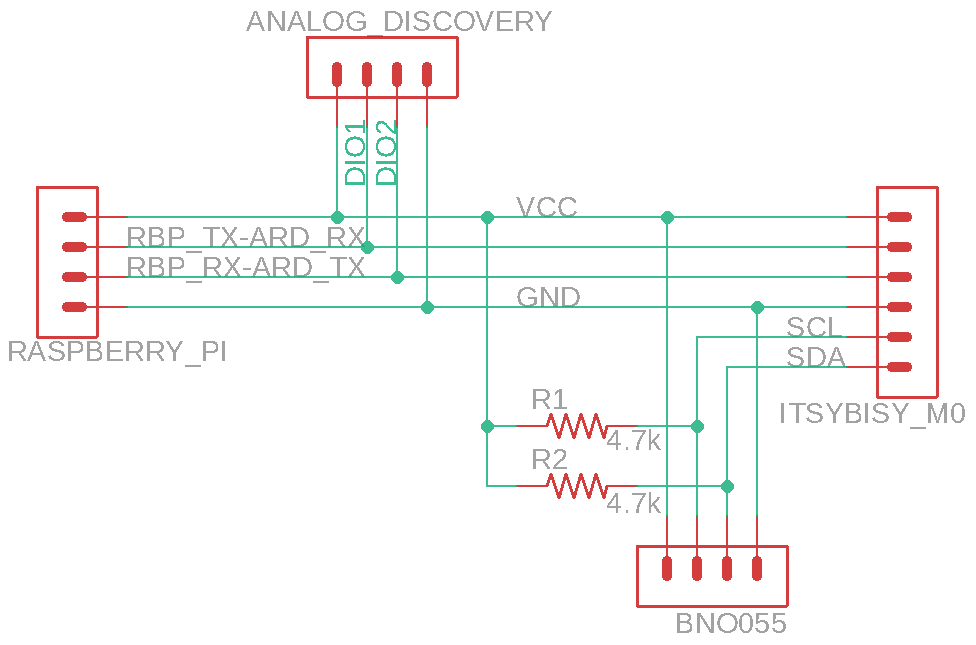
\includegraphics[width=\textwidth]{img/Lab3_SerialConnection.png}
		\caption{Circuit Diagram For Serial Connection} 
		\label{CNN4}
	\end{figure}
	\subsection{Procedure}
	To adapt the Arduino code, we first change our packet union definition to store an array of 10 floats and an array of 40 uint8\_ts instead of 1 and 4 respectively. Every 100 ms it then shifts the buffer to the right by one, and then replaces the first index of it with the new float. We will then utilize the send() method of PacketSerial to send this new packet to the Raspberry Pi. On the Raspberry Pi,  we simply read in the packet like before, except it is now read into an array, and every 4 bytes are converted into a float like the last experiment. The code changes for this experiment can be found in Appendix C.
	
	\subsection{Result}
	Now, every 100ms we can see the Arduino print out a value to the serial monitor, which is the new data point. However, only every 1 second can we see the data buffer on the Raspberry Pi. This buffer contains the last 10 data points collected by the Arduino.
	
	\clearpage
	\section{RPi ask for data using COBS PacketSerial}
	\subsection{Setup}
	The hardware requirement for this section is following:
	\begin{itemize}
		\item Raspberry
		\item BNO055
		\item Itsybisy M0
		\item Analog Discovery
	\end{itemize}
	Connect all the component base on the following diagram \ref{CNN2}.
	\begin{figure}[hb]
		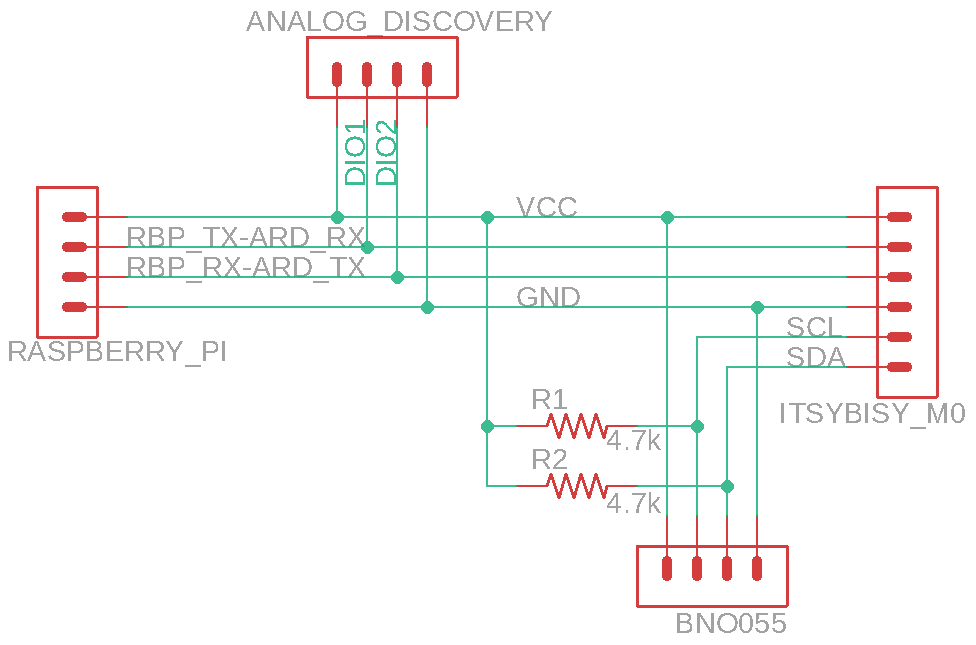
\includegraphics[width=\textwidth]{img/Lab3_SerialConnection.png}
		\caption{Circuit Diagram For Serial Connection} 
		\label{CNN2}
	\end{figure}
	\subsection{Procedure}
	The steps to finish the goal is following.
	\begin{itemize}
		\item Raspberry Pi need to send a message to Itsybisy to request data.
		\item Itsybisy need to read data Raspberry Pi ask for and package it base on the COB format
		\item Raspberry Pi need to read the COB data and change it back to float data and display it to the screen.
	\end{itemize}
	\subsubsection{Step one}
	Main program construct a data packet which contain data and length of this data. Serial handler will use the \textbf{serialPuts} function to put the data to serial buffer and let system send it.
	\begin{lstlisting}
	void send(Datapacket* p){
		serialPuts(fd,p->data);
		if (p->data[p->length-1]==0)
		{
			serialPutchar(fd,'\0');
		}
	
	}
	\end{lstlisting}
	\subsubsection{Step two}
	Itsybisy will receive the request and read the data from the BNO055.
	\begin{lstlisting}
	void loop() {
		myPacketSerial.update();
		if (myPacketSerial.overflow())
			Serial.println("Buffer Overflow!");
		for (int i = 0; i < 10; i++) {
			myPacketSerial.update();
			imu::Vector<3> accel = bno
			.getVector(Adafruit_BNO055::VECTOR_LINEARACCEL);
			
			float temp = pow(accel.x(), 2) 
				+ pow(accel.y(), 2) 
				+ pow(accel.z(), 2);
			float mag = sqrt(temp);
			if (mag - previousMag >= 2.0) {
				myPacketSerial.send(bumpPacket, 4);
			}
			previousMag = mag;
			Serial.print("Accelaration Magnitude: ");
			Serial.println(mag);
			addToBuffer(mag);
			
			
			/* Wait the specified delay before requesting nex data */
			delay(BNO055_SAMPLERATE_DELAY_MS);
		}
	}
	
	void onPacketReceived(const uint8_t* buffer, size_t size) {
		if (size==4&&compare(buffer,"test"))
			myPacketSerial.send(packet1.packet_data, 40);
	}
	
	bool compare(const uint8_t* buffer,const uint8_t* buffer2, int size){
		for (int i = 0; i < size; i++)
		{
			if(buffer[i]!=buffer2[i])return false;
		}
		return true;
	}
	
	void addToBuffer(float newMeasurement) {
		for (int i = 9; i >= 0; i--) {
			packet1.packet_float[i] = packet1.packet_float[i - 1];
		}
		packet1.packet_float[0] = newMeasurement;
	}
	\end{lstlisting}
	\subsubsection{Step three}
	Raspberry Pi will get the data and decode the format.
	\begin{lstlisting}
	void SerialHandler::operator >>(Datapacket* dp){
		int length=0;
		char buffer[40960];
			int isBegin=0;
		while (1)
		{
			if(isBegin==0){
				buffer[length]=(char)serialGetchar(fd);
				length++;
				usleep(100);
				if(buffer[length-1]==0){
					isBegin=0;
					break;
				}
			}
		}
		char* frame=new char[length];
		memcpy(frame,buffer,length);
		dp->data=frame;
		dp->length=length;
	}
	
	void COBHandler::operator>= (Datapacket* p){
		char* rawData=p->data;
		int index=0;
		int nextIndex=0;
		while (index<p->length-1){
			nextIndex=(uint16_t)rawData[index];
			rawData[index]=0;
			index+=nextIndex;
		}
		char* newData=new char[p->length-2];
		memcpy(newData,rawData+1,p->length-2);
		p->length-=2;
		p->data=newData;
	} 
	\end{lstlisting}
	\subsection{Result}
	When the raspberry pi send the request\ref{ana_ardu}, arduino read the data from BNO055 and send to raspberry pi. Raspberry Pi decode it and display it to the screen\ref{rbp_data}.
	\begin{figure}[hb]
		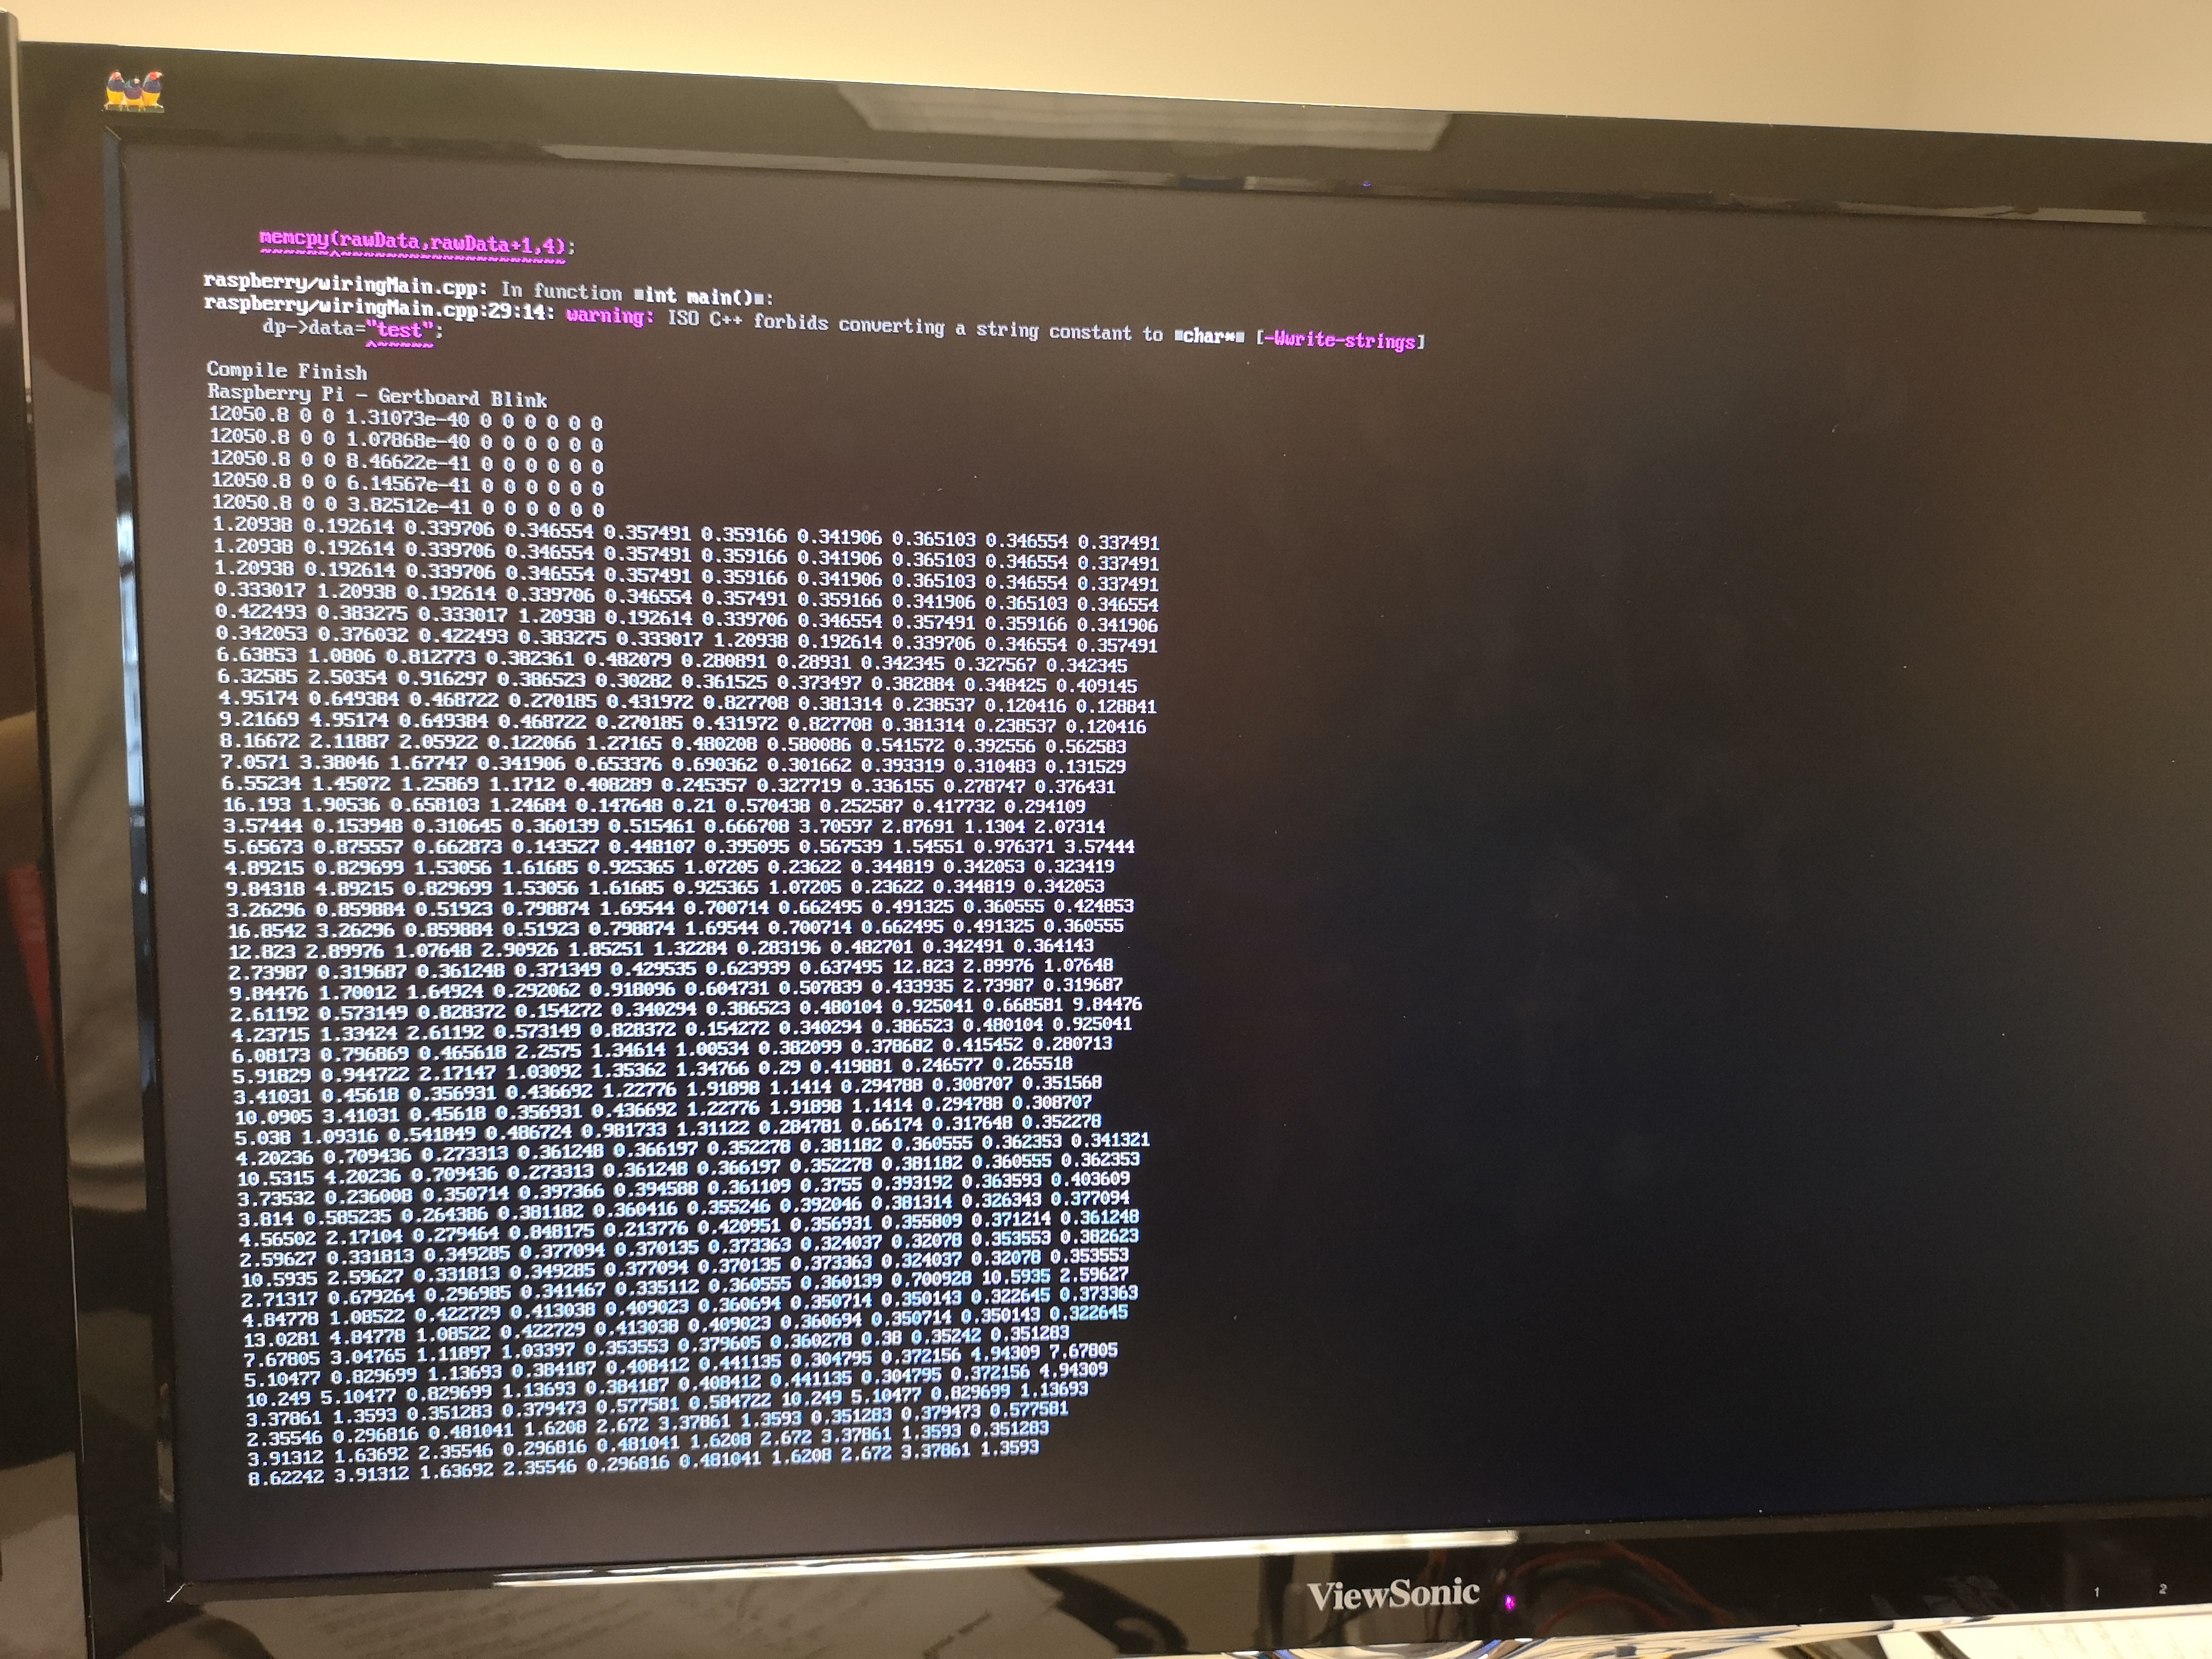
\includegraphics[width=\textwidth]{img/Lab2_Arduino-rbp_1.jpg}
		\caption{Data Received by Raspberry Pi} 
		\label{rbp_data}
	\end{figure}
	\begin{figure}[hb]
		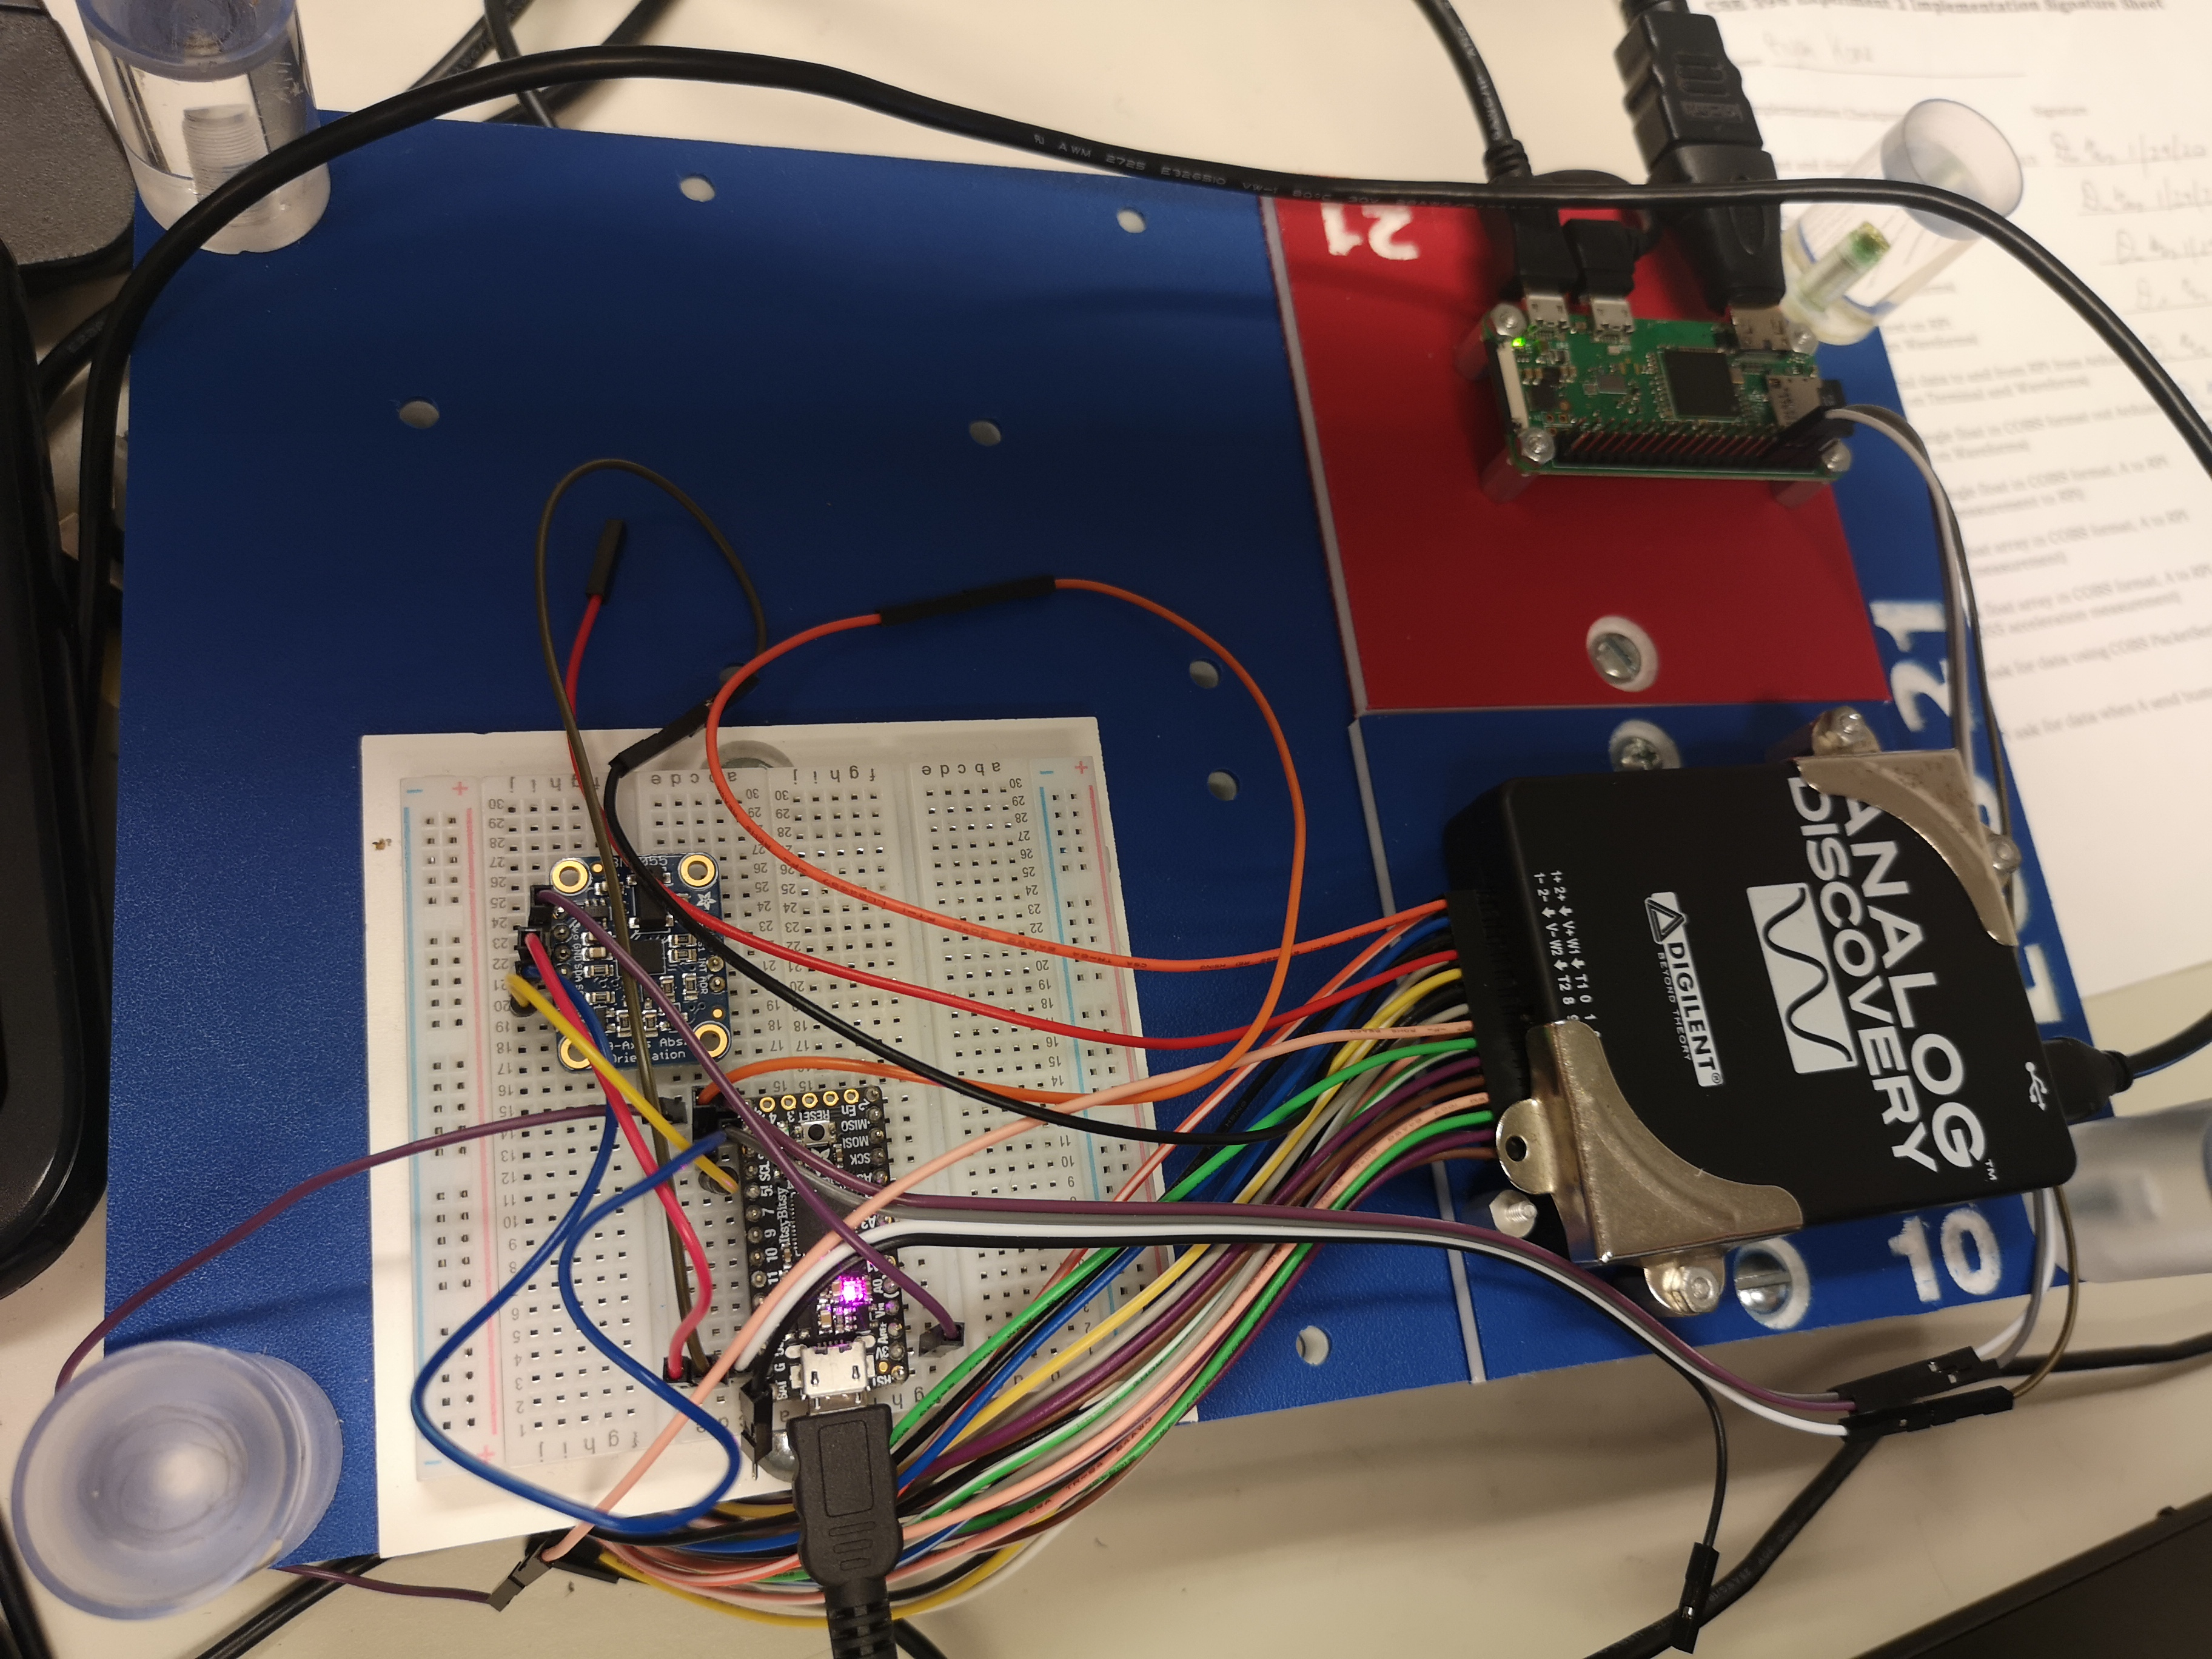
\includegraphics[width=\textwidth]{img/Lab2_Arduino-rbp_2.jpg}
		\caption{Physical Connection} 
		\label{ana_ardu}
	\end{figure}
	\clearpage
	\section{RPi ask for data when A send bump detected}
	\subsection{Setup}
	The hardware requirement for this section is following:
	\begin{itemize}
		\item Raspberry
		\item BNO055
		\item Itsybisy M0
		\item Analog Discovery
	\end{itemize}
	Connect all the component base on the following diagram \ref{CNN1}.
	\begin{figure}[hb]
		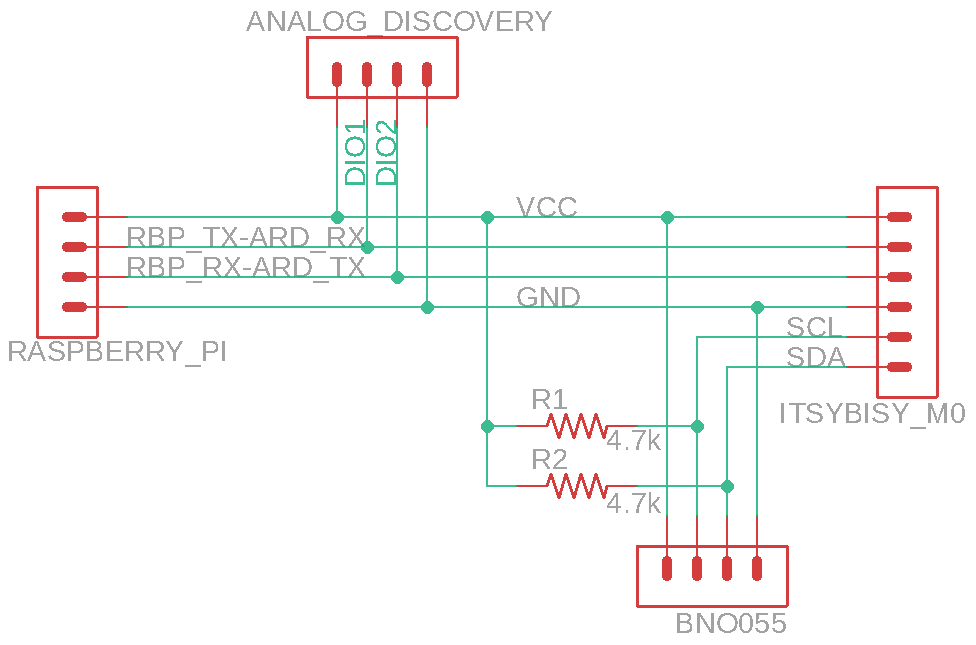
\includegraphics[width=\textwidth]{img/Lab3_SerialConnection.png}
		\caption{Circuit Diagram For Serial Connection} 
		\label{CNN1}
	\end{figure}
	\subsection{Procedure}
		The steps to finish the goal is following.
	\begin{itemize}
		\item Itsybisy detect a bump and send a event to Raspberry Pi
		\item Raspberry Pi need to send a message to Itsybisy to request data.
		\item Itsybisy need to read data Raspberry Pi ask for and package it base on the COB format
		\item Raspberry Pi need to read the COB data and change it back to float data and display it to the screen.
	\end{itemize}
	\subsubsection{Step one}
	Itsybisy will reading the data and send a message to Raspberry Pi when it detect the data have a bump.
	\begin{lstlisting}
	void loop() {
		myPacketSerial.update();
		if (myPacketSerial.overflow()) {
			Serial.println("Buffer Overflow!");
		}
		for (int i = 0; i < 10; i++) {
			myPacketSerial.update();
			imu::Vector<3> accel = bno.getVector(Adafruit_BNO055::VECTOR_LINEARACCEL);
			
			float temp = pow(accel.x(), 2) + pow(accel.y(), 2) + pow(accel.z(), 2);
			float mag = sqrt(temp);
			if (mag - previousMag >= 2.0) {
				myPacketSerial.send(bumpPacket, 4);
			}
			previousMag = mag;
			Serial.print("Accelaration Magnitude: ");
			Serial.println(mag);
			addToBuffer(mag);
			
			
			/* Wait the specified delay before requesting nex data */
			delay(BNO055_SAMPLERATE_DELAY_MS);
		}
	}
	\end{lstlisting}
	\subsubsection{Step two}
	Main program construct a data packet which contain data and length of this data. Serial handler will use the \textbf{serialPuts} function to put the data to serial buffer and let system send it.
	\begin{lstlisting}
	void send(Datapacket* p){
		serialPuts(fd,p->data);
		if (p->data[p->length-1]==0)
		{
			serialPutchar(fd,'\0');
		}
	
	}
	\end{lstlisting}
	\subsubsection{Step three}
	Itsybisy will receive the request and read the data from the BNO055.
	\begin{lstlisting}
	void loop() {
		myPacketSerial.update();
		if (myPacketSerial.overflow())
		Serial.println("Buffer Overflow!");
		for (int i = 0; i < 10; i++) {
			myPacketSerial.update();
			imu::Vector<3> accel = bno
			.getVector(Adafruit_BNO055::VECTOR_LINEARACCEL);
			
			float temp = pow(accel.x(), 2) 
			+ pow(accel.y(), 2) 
			+ pow(accel.z(), 2);
			float mag = sqrt(temp);
			if (mag - previousMag >= 2.0) {
				myPacketSerial.send(bumpPacket, 4);
			}
			previousMag = mag;
			Serial.print("Accelaration Magnitude: ");
			Serial.println(mag);
			addToBuffer(mag);
			
			
			/* Wait the specified delay before requesting nex data */
			delay(BNO055_SAMPLERATE_DELAY_MS);
		}
	}
	
	void onPacketReceived(const uint8_t* buffer, size_t size) {
		if (size==4&&compare(buffer,"test"))
			myPacketSerial.send(packet1.packet_data, 40);
	}
		
	bool compare(const uint8_t* buffer,const uint8_t* buffer2, int size){
		for (int i = 0; i < size; i++)
		{
			if(buffer[i]!=buffer2[i])return false;
		}
		return true;
	}
	
	void addToBuffer(float newMeasurement) {
		for (int i = 9; i >= 0; i--) {
			packet1.packet_float[i] = packet1.packet_float[i - 1];
		}
		packet1.packet_float[0] = newMeasurement;
	}
	\end{lstlisting}
	\subsubsection{Step four}
	Raspberry Pi will get the data and decode the format.
	\begin{lstlisting}
	void SerialHandler::operator >>(Datapacket* dp){
		int length=0;
		char buffer[40960];
		int isBegin=0;
		while (1)
		{
			if(isBegin==0){
				buffer[length]=(char)serialGetchar(fd);
				length++;
				usleep(100);
				if(buffer[length-1]==0){
					isBegin=0;
					break;
				}
			}
		}
		char* frame=new char[length];
		memcpy(frame,buffer,length);
		dp->data=frame;
		dp->length=length;
	}
	
	void COBHandler::operator>= (Datapacket* p){
		char* rawData=p->data;
		int index=0;
		int nextIndex=0;
		while (index<p->length-1){
			nextIndex=(uint16_t)rawData[index];
			rawData[index]=0;
			index+=nextIndex;
		}
		char* newData=new char[p->length-2];
		memcpy(newData,rawData+1,p->length-2);
		p->length-=2;
		p->data=newData;
	} 
	\end{lstlisting}
	\subsection{Result}
	When itsybisy detect a bump, it send a event Raspberry Pi \ref{ana_ardu3} and Raspberry Pi request the data from the itsybisy \ref{rbp_data3}. Raspberry Pi decode it and display in the screen \ref{ana_ardu2} \ref{rbp_data2}.
	\begin{figure}[hb]
		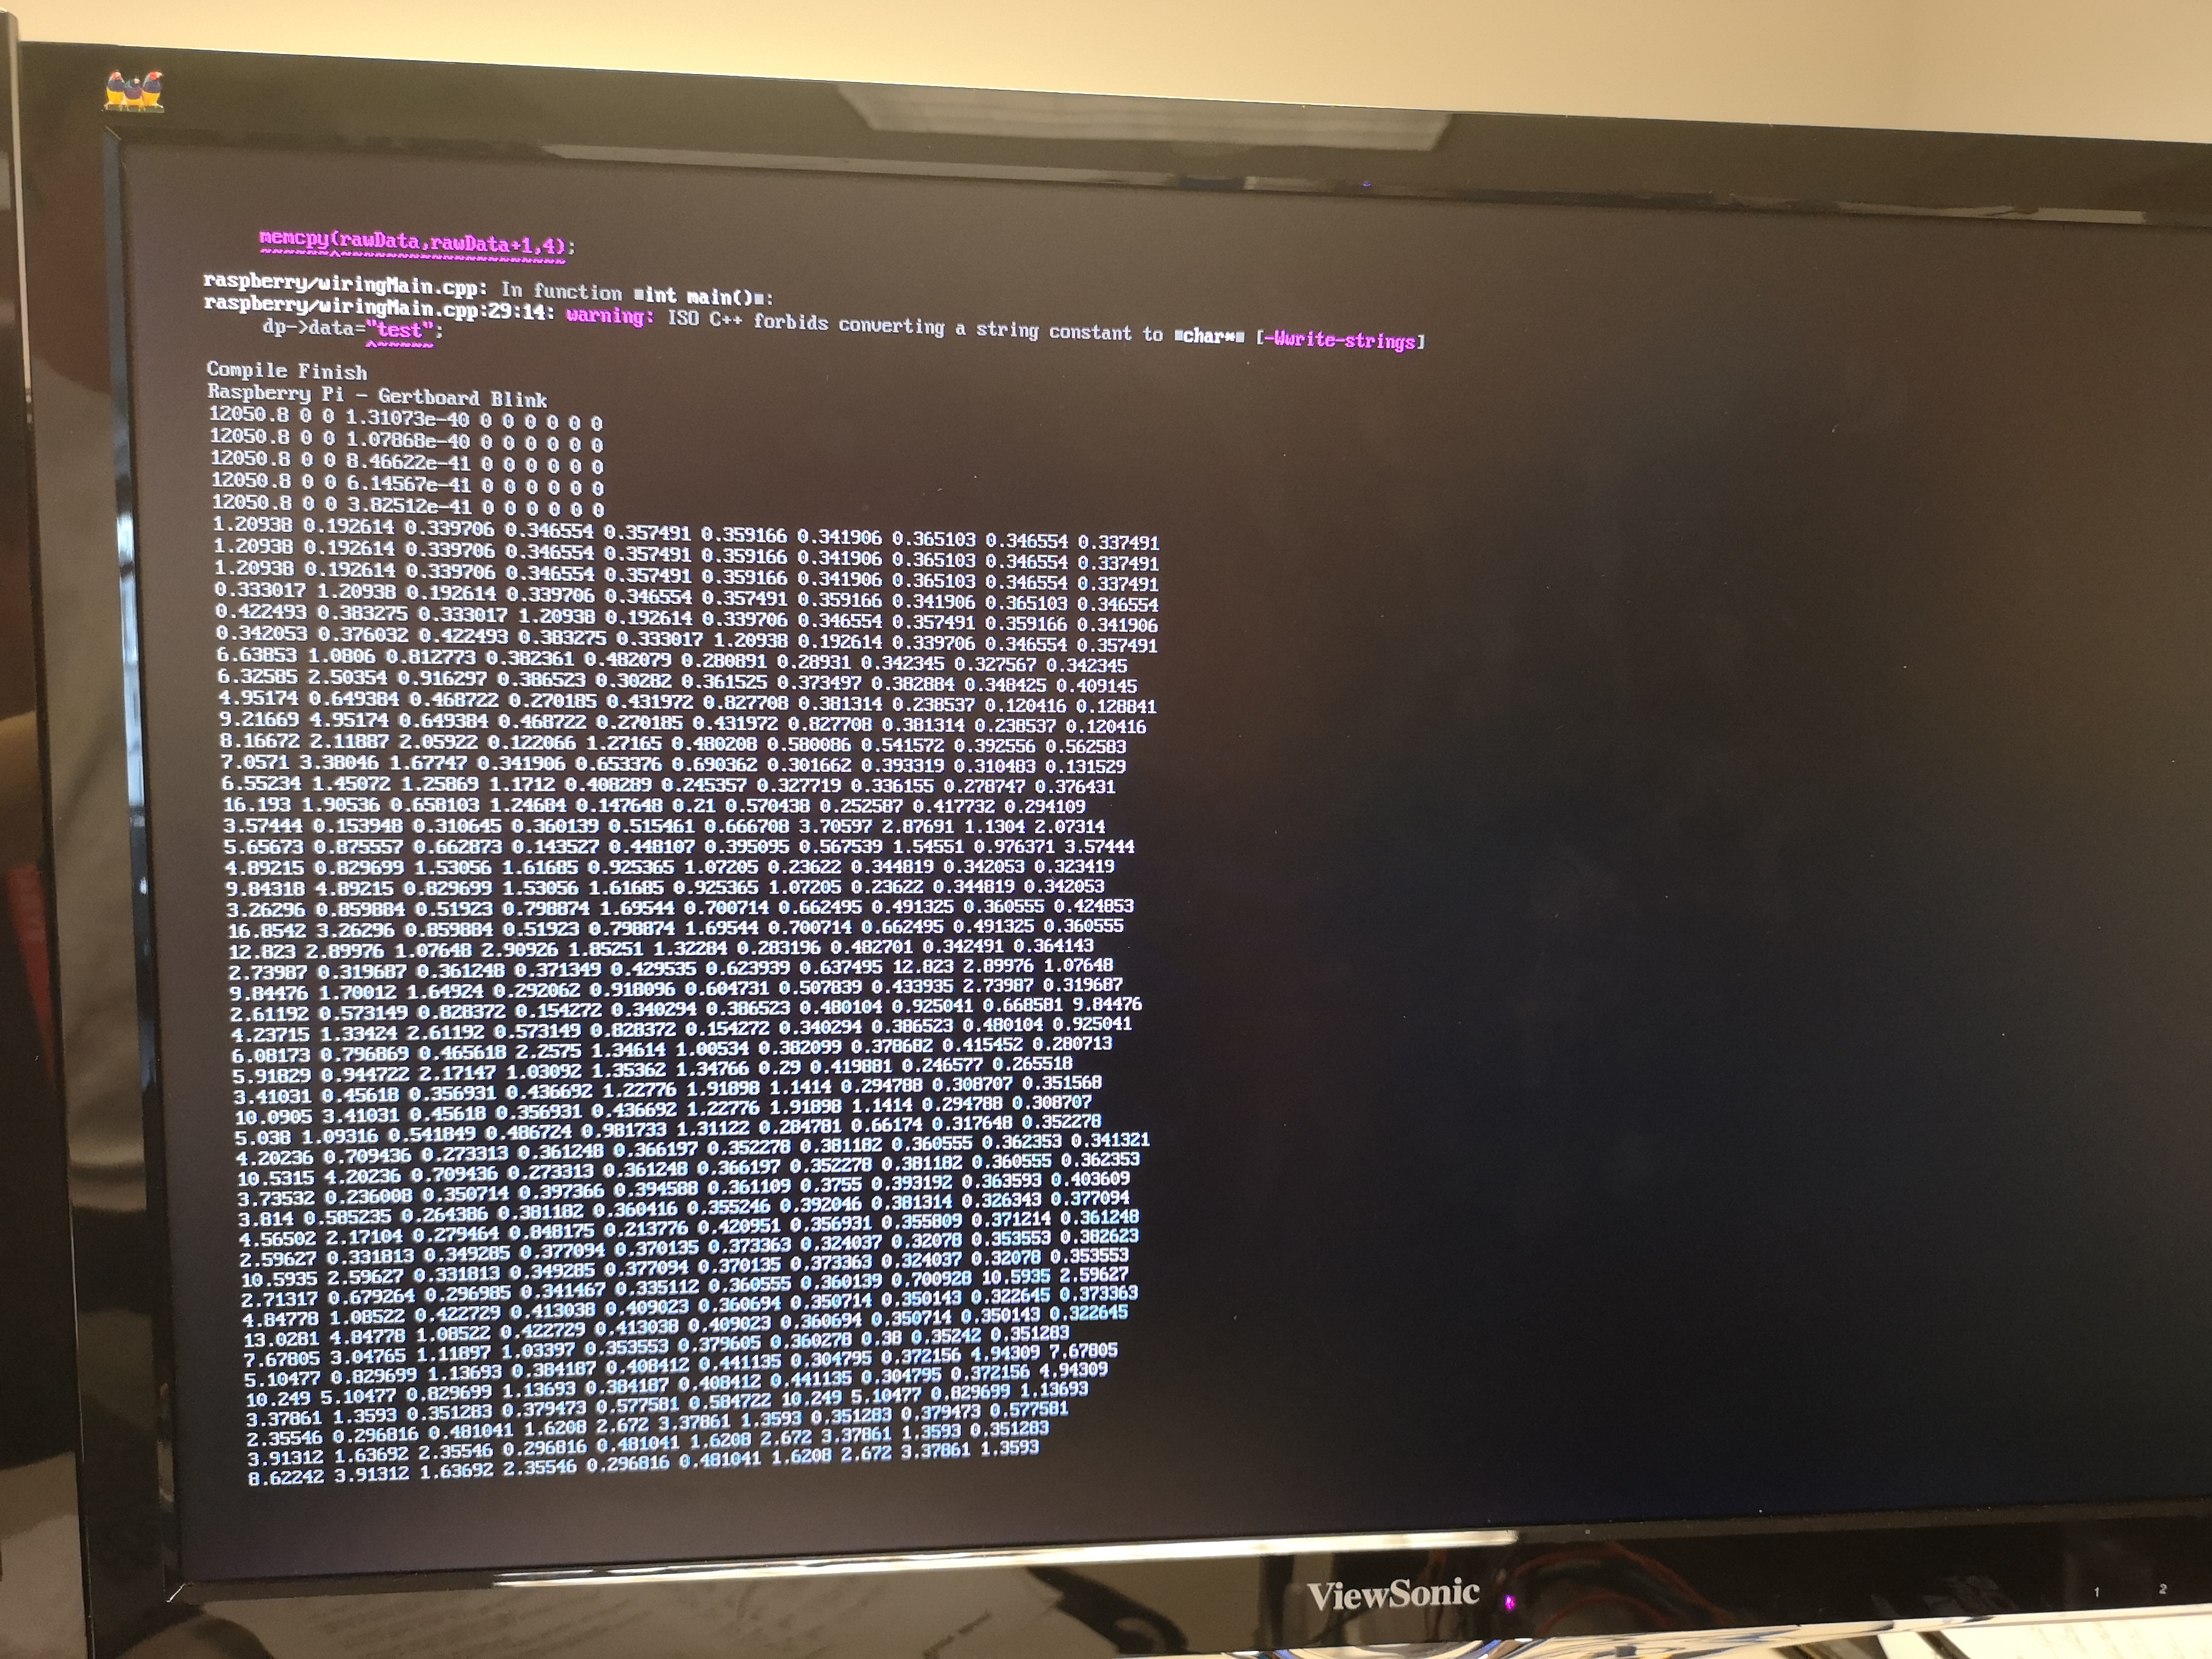
\includegraphics[width=\textwidth]{img/Lab2_Arduino-rbp_1.jpg}
		\caption{Data Received by Raspberry Pi} 
		\label{rbp_data2}
	\end{figure}

	\begin{figure}[hb]
		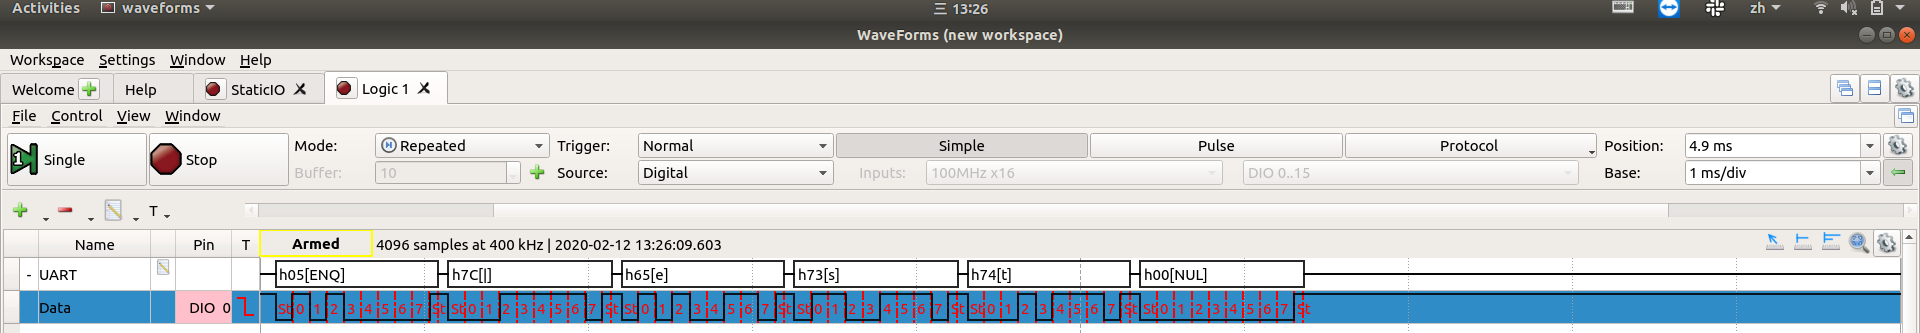
\includegraphics[width=\textwidth]{img/Lab2_RBP_Data.png}
		\caption{Data Send by Raspberry Pi} 
		\label{rbp_data3}
	\end{figure}

	\begin{figure}[hb]
		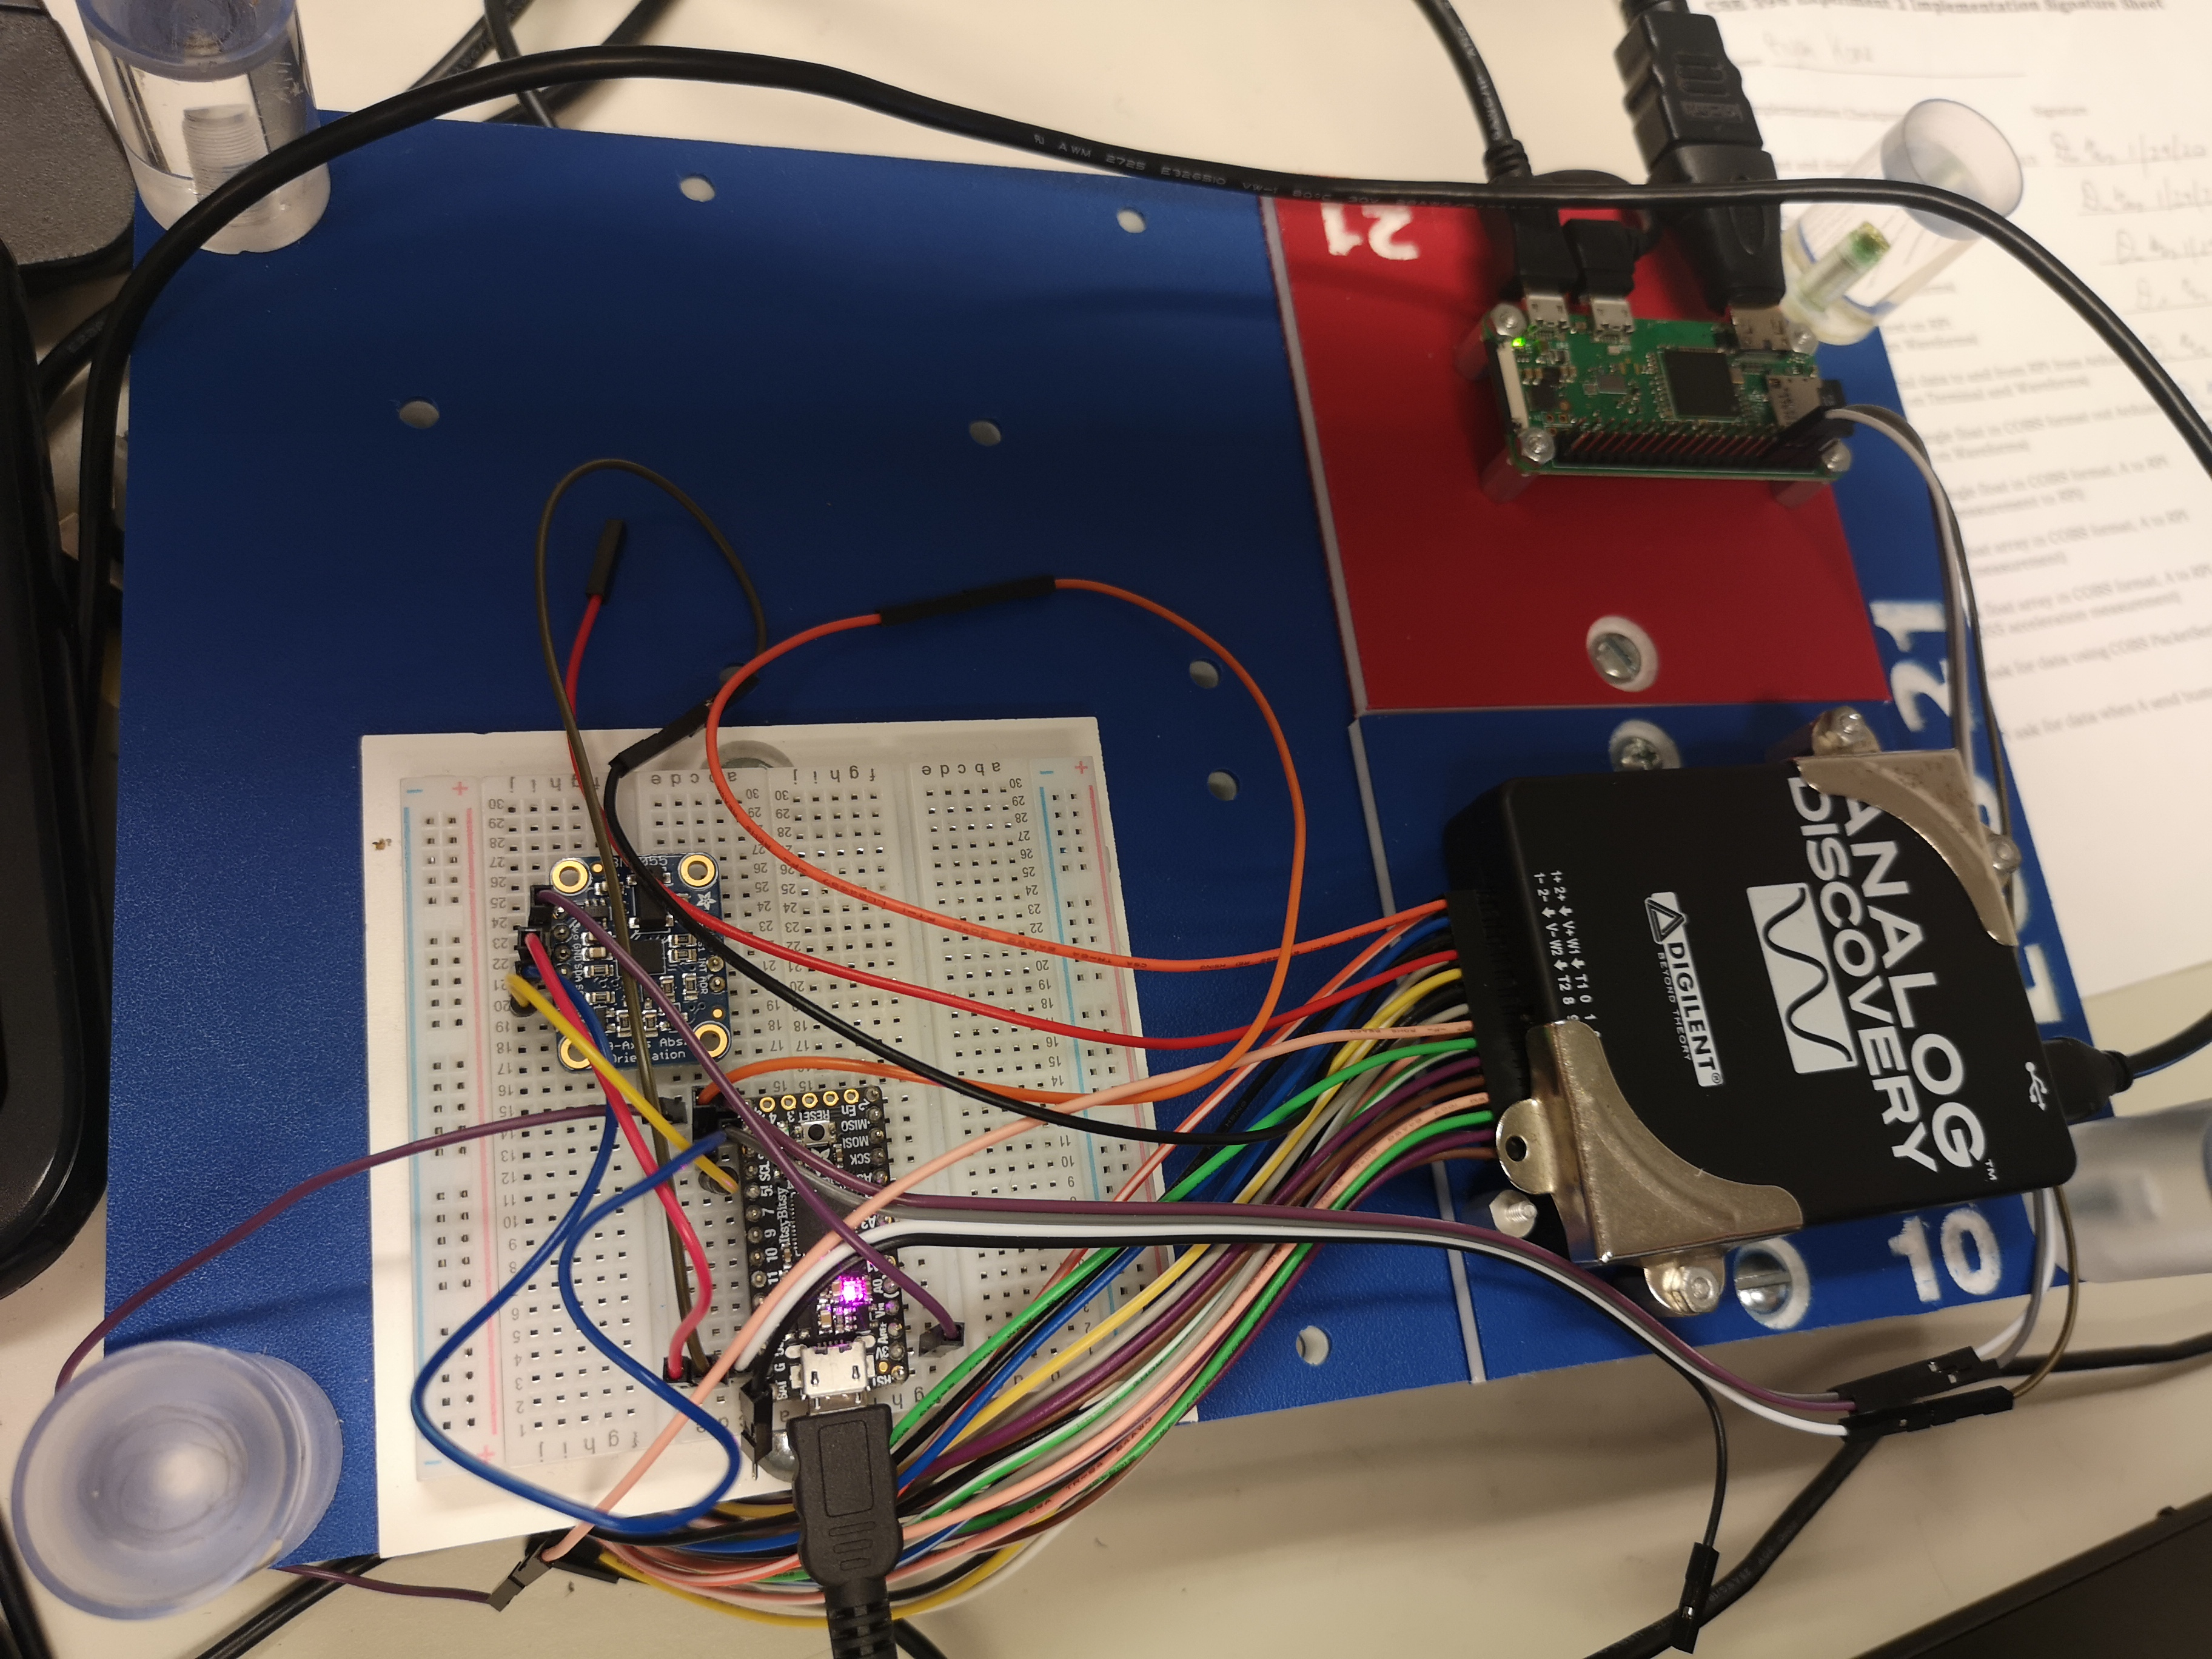
\includegraphics[width=\textwidth]{img/Lab2_Arduino-rbp_2.jpg}
		\caption{Physical Connection} 
		\label{ana_ardu2}
	\end{figure}
	\begin{figure}[hb]
		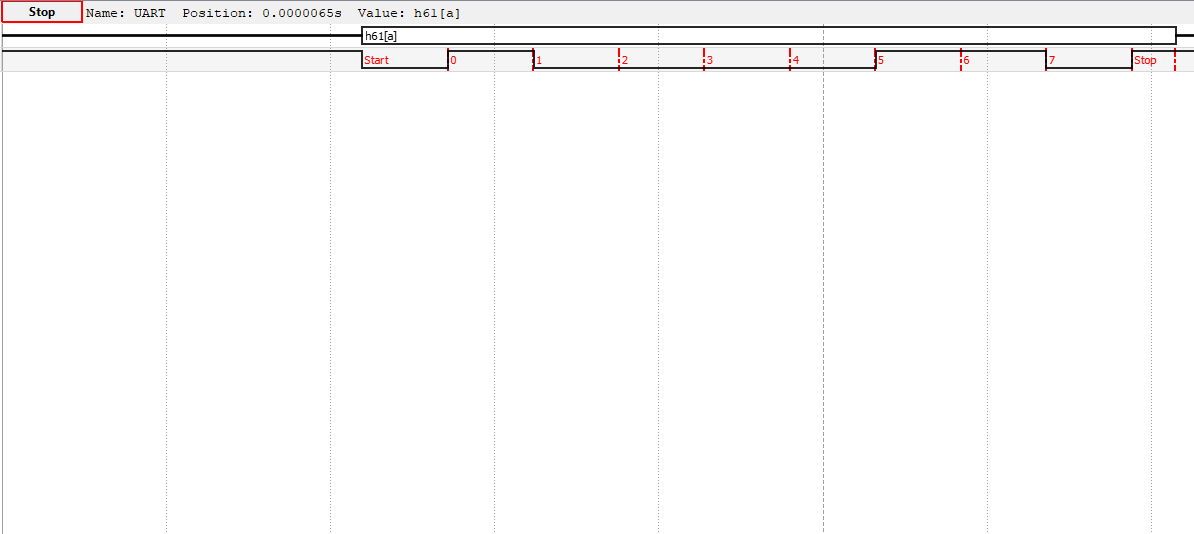
\includegraphics[width=\textwidth]{img/Lab3_ArduinosendChar.PNG}
		\caption{Analog Discovery Logic Itsybisy Serial} 
		\label{ana_ardu3}
	\end{figure}
	\clearpage
	\section{Conclusion}
	By using the open source hardware and COB encoding method, we create a embedded system which can detect a bump to table and record the data about this event. During development, we discover the computer system which not as powerful as a PC still will be able to do variety of tasks.
	\section{Appendix}
	\subsection{Appendix A}
	\begin{lstlisting}
		#include "PacketSerial.h" 
		
		PacketSerial_<COBS, 0, 255> myPacketSerial;  
		uint8_t myPacket[3] = { 1, 0, 1 }; 
		
		void setup() { 
		Serial1.begin(9600); 
		myPacketSerial.setStream(&Serial1); 
		myPacketSerial.setPacketHandler(&onPacketReceived); 
		} 
		
		void loop() { 
		myPacketSerial.update(); 
		myPacketSerial.send(myPacket, 3); 
		delay(1000); 
		}
	\end{lstlisting}
	\subsection{Appendix B}
	\begin{lstlisting}
	#include "PacketSerial.h" 
	
	PacketSerial_<COBS, 0, 255> myPacketSerial; 
	
	typedef union _packet { 
		float packet_float; 
		uint8_t data[4]; 
	}; 
	
	_packet packet1; 
	
	void setup() { 
		Serial.begin(9600); 
		pinMode(A1, INPUT); 
		Serial1.begin(9600); 
		myPacketSerial.setStream(&Serial1); 
		myPacketSerial.setPacketHandler(&onPacketReceived); 
	} 
	
	void loop() { 
		packet1.packet_float = (analogRead(A1) / 1024.0) * 3; 
		myPacketSerial.update(); 
		myPacketSerial.send(packet1.data, 4); 
	}
	\end{lstlisting}
		\subsection{Appendix C}
	\begin{lstlisting}
	#include "PacketSerial.h"
	
	PacketSerial_<COBS, 0, 255> myPacketSerial;
	
	
	typedef union _packet {
		float packet_float[10];
		uint8_t packet_data[40];
	};
	
	_packet packet1;
	
	
	void setup() {
		Serial.begin(9600);
		pinMode(A1, INPUT);
		Serial1.begin(9600);
		myPacketSerial.setStream(&Serial1);
		myPacketSerial.setPacketHandler(&onPacketReceived);
	}
	
	void loop() {
		for(int i = 0; i < 10; i++) {
			addToBuffer((analogRead(A1) / 1024.0) * 3.0);
			myPacketSerial.update();
			delay(100);
		}
		printPacket(packet1);
		myPacketSerial.send(packet1.packet_data, 40);
	}
	
	void addToBuffer(float newMeasurement) {
		for (int i = 9; i >= 0; i--) {
			packet1.packet_float[i] = packet1.packet_float[i - 1];
		}
		packet1.packet_float[0] = newMeasurement;
	}
	\end{lstlisting}
\end{document}